\chapter{Ownership, Scale, and Market Judgment}

This lecture begins with outcomes rather than first principles. We are shown exits at large scale, nine-figure wealth, and a series of short interviews staged on golf courses, and only afterward are we allowed to ask what mechanisms could have produced those outcomes. The chapter follows that spoken progression. We move from wealth as headline quantity to wealth as structure: ownership rather than wages, maturity matching rather than careless leverage, replication rather than improvisation, constraint rather than mere ambition, and finally the psychology by which markets and public narratives distort judgment.

\begin{remark}
No validated blackboard images survive for this lecture. The formulas in this chapter are therefore careful transcript-based reconstructions of the commercial logic stated in the interviews, not transcriptions of visible board equations.
\end{remark}

\section{Opening Stakes}

The opening montage functions like boundary data. Before any argument is made, the speaker places on the table a few scale markers:
\begin{equation}
V_1 \approx \$25\,\mathrm{M}, \qquad
V_2 \approx \$200\,\mathrm{M}, \qquad
V_{\mathrm{buyer,now}} \approx \$10\,\mathrm{B}.
\end{equation}
Alongside this comes a personal wealth claim,
\begin{equation}
NW \approx \$110\,\mathrm{M},
\end{equation}
and a teaser about hostility toward billionaires. None of this yet explains anything. It merely sets the size of the phenomenon to be explained.

This is the right way to hear the opening. The lecture does not say: here is a general theorem of wealth creation. It says instead: here are people who have reached conspicuous commercial outcomes; let us now ask, in public and in sequence, what habits, structures, and judgments lie underneath.

The golf-course framing matters because it turns the problem from abstract self-help into field observation. The premise is simple: if deals and networks concentrate in certain places, then advice may also concentrate there. The lecture therefore begins with a search procedure before it gives us a doctrine.

\section{Equity, Financing, and Integrity}

The first substantial interview begins socially and then tightens quickly. We hear what the men did for a living---oil and gas, banking, real estate---but the conversation does not stay at the level of profession. It moves almost immediately to mechanism: what in a competitive business actually produces wealth?

A compact way to preserve the first answer is the following table.
\begin{table}[h]
\centering
\begin{tabular}{ll}
\textbf{Instrument} & \textbf{Role in the lecture} \\
Salary $S$ & funds present living and stability \\
Equity $E$ & carries upside and accumulates wealth
\end{tabular}
\caption{Transcript-based compression of the first interview's wealth distinction.}
\end{table}

The speaker's claim is not that salary is useless. On the contrary, salary is what lets one live. The sharper claim is that salary does not usually provide the convexity required for large wealth. As a minimal reconstruction, we may write
\begin{equation}
W \approx S_{\mathrm{saved}} + \Delta E,
\end{equation}
where $W$ is accumulated wealth, $S_{\mathrm{saved}}$ is the portion of salary not consumed, and $\Delta E$ is the change in equity value. The asymmetry is the point: for large outcomes, the lecture places the real weight on $\Delta E$.

\subsection{Question \& Answer}

\paragraph{Question.} Why does equity build wealth better than salary?

\paragraph{Answer.} Because salary is linear and immediate, while ownership participates in the growth of the asset itself. A wage pays for the present. Equity places us on the balance-sheet side of the business, where appreciation, resale, and scale accrue. The first interview states this in ordinary language: one may live off salary, but wealth is built by owning a piece of what one works on.

Once ownership is introduced, the lecture does something important: it does not romanticize it. It immediately adds a structural condition. Long-duration bets require long-duration funding:
\begin{equation}
T_{\mathrm{finance}} \gtrsim T_{\mathrm{venture}}.
\end{equation}

\begin{proposition}
If a venture has a long payoff horizon but is financed with short-term money, control of the venture is exposed to refinancing risk before the venture matures.
\end{proposition}

\begin{proof}
Let $T_{\mathrm{venture}}$ denote the time over which the investment must develop before its value is realized, and let $T_{\mathrm{finance}}$ denote the maturity of the funding used to carry it. If $T_{\mathrm{finance}} < T_{\mathrm{venture}}$, the capital structure must be renewed before the business logic has finished unfolding. If renewal fails, becomes expensive, or comes with harsher terms, the underlying asset may have to be sold or surrendered while still midstream. This is exactly the warning given in the interview: short-term money on a long-term venture can get the whole thing taken away.
\end{proof}

The final move in this first interview is characterological. After ownership and financing, the lecture asks what trait successful people share. The answer is integrity. In context this is not moral decoration. It is a practical claim about commercial trust. If ownership creates upside and maturity matching preserves the venture in time, integrity preserves the willingness of others to transact with us at all.

\section{From Diversification to Concentration}

The lecture then pivots from compact maxims on the course to a more extended case study at a mansion. This shift in scale is deliberate. We are no longer collecting short principles from several men; we are now tracing one operating path from industry entry to nine-figure outcome.

The entrepreneur describes a path through medical device sales, then distributorship, and then founding his own company. The central contrast here is between two investment doctrines. Stockbroker training taught diversification. The billionaire advice he later heard in executive programs said almost the opposite: if one finds something one truly believes in, one may put concentrated effort and capital into that one thing and grow it.

The lecture does not turn this into a universal law. It presents it as a case-dependent doctrine of conviction and control. Concentration makes sense here because the entrepreneur is not merely buying an outside asset; he is building and governing the very business into which the capital goes. That is why self-funding matters in the spoken sequence. The logic is not only concentration, but concentration plus operational authority.

This is the place where the lecture moves from wealth \emph{capture} to wealth \emph{construction}. Ownership in the first interview was already important, but here ownership is coupled to control, and control is coupled to the business one is actively scaling.

\section{Turnkey Scale and the Logic of Replication}

When the lecture asks how the business moved from eight figures to nine, the answer is not mystical. It is procedural. The entrepreneur cites the idea of a turnkey method: prove the model, then duplicate it. His own phrasing---``copy, paste, copy, paste''---is the right rhythm to preserve.

A compact numerical summary is
\begin{equation}
N_{\mathrm{states}} : 1 \rightarrow 43.
\end{equation}
The business begins with one-state validation in California and then expands to $43$ states by repeating a package rather than reinventing the business anew in each place.

\begin{figure}[h]
\centering
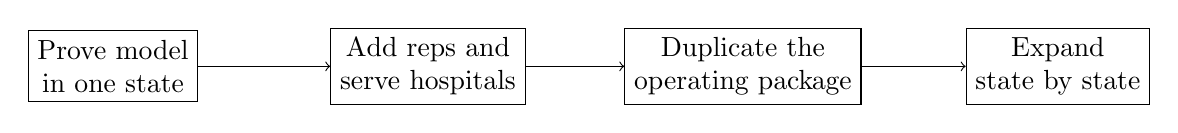
\begin{tikzpicture}
\node[draw, rectangle, align=center] (a) at (0,0) {Prove model\\in one state};
\node[draw, rectangle, align=center] (b) at (4,0) {Add reps and\\serve hospitals};
\node[draw, rectangle, align=center] (c) at (8,0) {Duplicate the\\operating package};
\node[draw, rectangle, align=center] (d) at (12,0) {Expand\\state by state};
\draw[->] (a) -- (b);
\draw[->] (b) -- (c);
\draw[->] (c) -- (d);
\end{tikzpicture}
\caption{Editorial schematic of the replication logic described in the interview.}
\end{figure}

What matters here is that scale appears as a controlled repetition of a previously validated unit. The lecture does not describe growth as charisma, nor as a vague exhortation to hustle. It describes growth as the repeated application of a working form.

\subsection{Question \& Answer}

\paragraph{Question.} How can growth itself almost kill a successful company?

\paragraph{Answer.} Because growth is not only revenue. It is also production, delivery, inventory, and working capital. If the demand side outruns the capacity side, success can become the mechanism of distress.

A small update model captures the logic:
\begin{align}
B_{t+1} &= B_t + Q_t - C_t,\\
K^{\mathrm{req}}_{t+1} &= k\,B_{t+1}.
\end{align}
Here $Q_t$ is incoming demand, $C_t$ is productive capacity, $B_t$ is backlog, and $k$ is working capital required per unit of unresolved production. If $Q_t > C_t$ for several periods, then backlog rises; as backlog rises, required working capital rises with it.

The entrepreneur's warning may then be written schematically as
\begin{equation}
g_{\mathrm{sales}} > g_{\mathrm{capacity}}
\;\land\;
K_t < K_t^{\mathrm{req}}
\;\Rightarrow\;
\text{growth distress}.
\end{equation}
This is the commercial meaning of the line that more companies die from indigestion than starvation. The firm did not fail because demand vanished. It nearly failed because demand arrived faster than the business could productively and financially absorb.

We should notice how disciplined the sequence is. First the lecture gives us the replication rule. Only afterward does it show us the hidden constraint. The entrepreneur is not retracting the scaling logic. He is bounding it.

\section{Product Discovery, Iteration, and the Sponsor Interruption}

After the low point, the lecture asks a better question: how does one find the winning product in the first place? The answer is cumulative rather than sudden.

\begin{enumerate}
\item Spend repeated time with the actual buyers and users---here, doctors and surgery centers.
\item Identify a neglected or under-attacked problem.
\item Improve the product incrementally over long periods.
\item Reach a tipping point at which the market begins to ask for the product rather than needing to be persuaded into it.
\end{enumerate}

That last shift is crucial. In the speaker's phrasing, it becomes fun when one is no longer making sales calls in the old sense, because people want the device after hearing about it. In commercial terms, the lecture is describing a transition from outbound push to inbound pull.

The narrator then recaps this for us. He says, in effect, that years of back-and-forth with prospective clients led to concrete solutions, and concrete solutions led to products that sold for millions and supported a nine-figure enterprise. The recap matters because it translates biography into mechanism.

\paragraph{Sponsor Interruption.} At this point the lecture is interrupted by a sponsor segment about communication automation. Since the argument is structurally separate from the interviews, we keep it separate here as well. The numerical claims are
\begin{equation}
p_{\mathrm{auto}} \le 90\%, \qquad
p_{\mathrm{cost\,reduction}} \approx 30\%.
\end{equation}
These figures belong to the ad copy, not to the core business doctrine of the chapter. They continue the video's general rhetoric of leverage, but they should not be treated as established operating results within the lecture itself.

\section{Opportunity, Public Narratives, and Market Psychology}

The final stretch of the lecture returns to the golf course and widens the frame. The speaker who sold companies for large sums is asked what he would tell his younger self. The first answer is ``don't waste time.'' From there the lecture broadens into a civic claim: America is presented as an opportunity field, not because outcomes are equal, but because entry is open enough that disciplined people can move.

This argument is then supported, in the speaker's own rhetoric, by a few public numbers:
\begin{equation}
p_{\mathrm{free\,enterprise}} \approx 87\%, \qquad
N_{\mathrm{billionaires}} \approx 750, \qquad
N_{\mathrm{population}} \approx 350\times 10^6.
\end{equation}
These are not proved statistics in the lecture. They are parameters in an interviewee's defense of free enterprise against a culture that, in his view, has begun to resent large wealth without studying the surrounding facts. The line of thought is clear enough: in a society that endorses free enterprise, extreme commercial outcomes are not anomalies to be apologized for but one possible consequence of the rules of the game.

The lecture then shifts from public narratives to market narratives. In the final interview, a retired lawyer offers the familiar but difficult rule: be greedy when others are scared, and scared when others are greedy. The theory is old. The interesting part is the explanation of why it is so difficult in practice.

\subsection{Question \& Answer}

\paragraph{Question.} If the rule is to buy low and sell high, why do people so often do the opposite?

\paragraph{Answer.} Because crowd emotion reverses the timing of action. Near a top, rising prices make people feel late and therefore eager to participate; near a bottom, falling prices make people feel endangered and therefore eager to flee.

A minimal transcript-based rendering is
\begin{align}
\sigma_{\mathrm{fear}} &\Rightarrow \text{accumulate},\\
\sigma_{\mathrm{greed}} &\Rightarrow \text{de-risk}.
\end{align}
And the desired price relation is simply
\begin{equation}
P_{\mathrm{buy}} < P_{\mathrm{sell}}.
\end{equation}
The difficulty is that the crowd tends to push in the opposite temporal direction. The lecture therefore treats contrarian investing not as cleverness, but as emotional discipline.

The final sharp note comes with the contrast between book smarts and street smarts. The lawyer's rhetorical question---how often does one solve a differential equation in the real world?---should not be heard as contempt for thought. It is a reminder that commercial action requires situational reading, timing, and human judgment. The lecture repeatedly places practical intelligence ahead of abstract prestige, though not ahead of study itself. Indeed, the earlier speaker explicitly tells younger people to study before forming opinions.

\section{Summary}

The lecture begins with flashy numbers, but its real content is structural. Wealth comes, in these interviews, from ownership rather than wages alone, from financing matched to the duration of the venture, from concentrated control when conviction is high, from replication of a working model, from respect for operational bottlenecks, and from long iteration close to the customer.

By the end, the argument broadens. Commercial success is not only a matter of product and scale; it is also a matter of public philosophy and private psychology. The lecture asks us to think well about free enterprise, to distrust social-media simplifications, and to understand that the simple rule ``buy low, sell high'' is hard precisely because crowds do not feel simple when prices move. In that sense the chapter closes where it should: not with a slogan, but with a demand for steadiness in judgment.